We provide a novel approach to solve this open problem, and juxtaposes this approach and its experimental results against the current state-of-the-art models. We empirically demonstrate the separation of content and style spaces by demonstrating the inferred spaces of labeled sentences in a sentiment-transfer task, where the positive sentences in the test set are converted to equivalent sentences with a negative sentiment, and vice-versa.

This model is also generalizable using its standard implementation to problems involving multiple classes, like style transfer by authors, artists, topic etc.

Our model is built upon an autoencoder with a sequence-to-sequence (Seq2Seq) neural network \citep{sutskever2014sequence}, as described in Section \ref{ssec:seq2seq-objective}. This is the primary objective of the algorithm, whose objective function is to simply reconstruct the input text. We implement our model with both deterministic autoencoders \citep{baldi2012autoencoders} as well as variational autoencoders \citep{kingma2013auto}.

Then we introduce two auxiliary losses, multi-task loss and adversarial loss in Sections \ref{ssec:multitask-objective} and \ref{ssec:adversarial-style-objective}, respectively. In addition to these auxiliary losses, we propose a novel bag-of-words adversarial loss in Section \ref{ssec:adversarial-bow-objective}. This makes our model a dual-adversary model. Section \ref{ssec:generating-novel-text} presents the approach to transfer style in natural language generation.

Figures \ref{fig:model-overview-training} and \ref{fig:model-overview-inference} depict the training and generation processes of our approach.

\begin{figure}[ht]
	\centering
	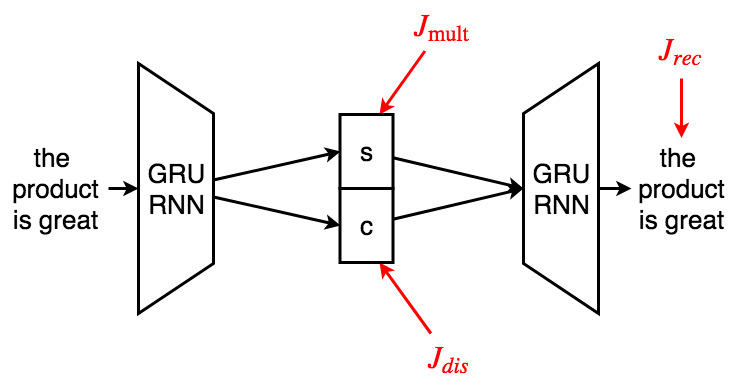
\includegraphics[width=\linewidth]{images/model-overview-training.png}
	\caption{Overview of Model Training}
	\label{fig:model-overview-training}
\end{figure}

\begin{figure}[ht]
	\centering
	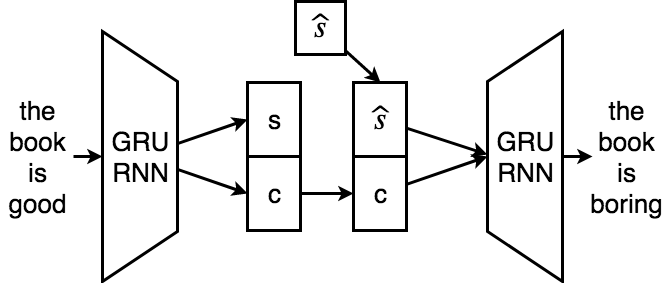
\includegraphics[width=\linewidth]{images/model-overview-inference.png}
	\caption{Overview of Model Inference}
	\label{fig:model-overview-inference}
\end{figure}


\section{Autoencoder} \label{ssec:seq2seq-objective}

An autoencoder encodes an input to a latent vector space, from which it decodes the input itself. By doing so, the autoencoder learns meaningful representations of data. This serves as our primary learning objective. Besides, we also use the autoencoder weights  for text generation in the attribute style-transfer application.

Let $x=(x_1, x_2, \cdots x_n)$ be an input sentence. The encoder encodes $x$ by a recurrent neural network (RNN) with gated recurrent units (GRU) \citep{cho2014learning}, and obtains a hidden state $\bm h$, which in our formulation, is two separate spaces, $\bm s$ for style and, $\bm c$ for content, which still requires an equivalent number of parameters compared to a vanilla RNN encoder.

Then a decoder RNN generates a sentence, which ideally should be $x$ itself. Suppose at a time step $t$, the decoder RNN predicts the word $x_t$ with probability $p(x_t | \bm h, x_1 \cdots x_{t-1})$, then the autoencoder is trained with cross-entropy loss, given by

First the encoder produces the style and content, given that $\theta_{E_s}$ represents the subset of encoder parameters responsible for the production of the style vector and $\theta_{E_c}$, similarly, represents the encoder responsible for the production of the content vector.
\begin{eqnarray} \label{eqn:dae-rec-1}
	\bm s &=& \theta_{E_s}(x) \nonumber \\
	\bm c &=& \theta_{E_c}(x) \nonumber
\end{eqnarray}

Following which the decoder attempts to predict the original distribution of $x$ by predicting the softmax over the vocabulary size, for as many time steps as the sequence length, as shown in Equation \ref{eqn:dae-rec-2}
\begin{equation} \label{eqn:dae-rec-2}
	\mathcal{L}_\text{rec}(\bm\theta_E,\bm\theta_D)= -\mathbb{E}[log p_D(x|\bm s, \bm c)]
\end{equation}
where $\bm\theta_E$ and $\bm\theta_D$ are the parameters of the encoder and decoder, respectively.

Since this loss trains the autoencoder to reconstruct $x$, it is also called the reconstruction loss.


\subsection{Variational Autoencoder}

In addition to the deterministic auto-encoding objective presented above, we also implement a variational autoencoder. The variational sampling and KL-divergence losses are applied for both the style space $\bm s$ and the content space $\bm c$. The weights applied to each KL-divergence loss is tuned independently as a hyperparameter.

Equation \ref{eqn:vae-rec} shows the reconstruction objective that is minimized by the model in the VAE variant of our model.

\begin{eqnarray} \label{eqn:vae-rec}
	\mathcal{L}_\text{rec}(\theta_D, \theta_E; x) &=& \nonumber
	- \mathbb{E}_{q_{E_s}(\bm s|x) q_{E_c}(\bm c|x)} [log p_D(x|\bm s, \bm c)] \nonumber \\ & &
	+ \lambda_{\text{skl}} KL(q_{E_s}(\bm s|x)||p(z)) \nonumber \\ & &
	+ \lambda_{\text{ckl}} KL(q_{E_c}(\bm c|x)||p(z))
\end{eqnarray}

The motivation for using a variational autoencoder variant to compare the base deterministic autoencoder model to, is the property of VAEs to learn smooth and continuous latent spaces, without many dead zones in the latent space that cannot be sampled from. \cite{bowman2016generating} show this empirically by using the latent space of a text variational autoencoder to interpolate between and generate novel sentences from the latent spaces between two valid sentences from a corpus.

Since our objective is to use empirically inferred latent vectors to eventually achieve the attribute style transfer objective, it would be beneficial to juxtapose the experimental performance of a variational autoencoder against a deterministic autoencoder.


Besides the above reconstruction losses, we design auxiliary losses to disentangle the latent space such that $\bm h$ can be separated into two spaces $\bm s$ and $\bm c$, representing style and content respectively, i.e., $\bm h = [\bm s ; \bm c]$, where $[\cdot;\cdot]$ denotes concatenation. We also design additional regularizations on the latent space to encourage learning this disentangled representation.


\todo[inline]{Re-write the next couple of sections for softmax classifiers}

\section{Multi-Task Loss} \label{ssec:multitask-objective}

Our first auxiliary loss ensures the style space does contain style information. We build a classifier on the style space $\bm s$ predicting the style label $y$, which is a part of the training data.

This loss can be viewed as a \textit{multi-task} loss, which makes the neural network not only decode the sentence, but also predicts its sentiment. Similar multi-task losses are used in previous work for sequence-to-sequence learning \citep{luong2015multi}, sentence representation learning \citep{jernite2017discourse} and sentiment analysis \citep{balikas2017multitask}, among others.

In our application, we follow previous work \citep{hu2017toward,shen2017style,fu2017style} and treat the sentiment as the style of interest. We introduce a binary classifier

\begin{equation}
	p(y|\bm s;\bm\theta_\text{mult})= softmax(\bm w_\text{mult}^\top \bm s + b_\text{mult})
\end{equation}
where $\bm\theta_\text{mult}=[\bm w_\text{mult}; b_\text{mult}]$ are the classifier's parameters for multi-task learning.

\begin{align} \label{eqn:multi-task-loss}
	 & \mathcal{L}_\text{mult}(\bm\theta_{E};\bm\theta_\text{mult})=      \\ \nonumber
	 & -s\log p_\text{mult}(s|\bm s) - (1-s)\log p_\text{mult}(1-s|\bm s)
\end{align}
where $\bm\theta_E$ are the encoder's parameters..


\section{Adversarial Style Discriminator} \label{ssec:adversarial-style-objective}

The above multi-task loss only operates on the style space, but does not have an effect on the content space $\bm c$.

We therefore apply an adversarial loss to disentangle the content space from style information, inspired by adversarial generation \citep{goodfellow2014generative}, adversarial domain adaptation \citep{liu2017adversarial}, and adversarial style transfer \citep{fu2017style}.

The idea of adversarial loss is to introduce an adversary that deliberately discriminates style $s$ on the content vector $\bm c$. Then the autoencoder is trained to learn such a content vector space that its adversary cannot predict style information.

Concretely, the adversarial discriminator predicts style $s$ by a logistic regression
\begin{equation}
	p_\text{dis}(s=1|\bm c;\bm\theta_\text{adv})=\sigma(\bm w_\text{adv}^\top \bm c + b_\text{adv})
\end{equation}
where $\bm\theta_\text{dis}=[\bm w_\text{dis}; b_\text{dis}]$ are the parameters of the adversary. It is trained by
\begin{align}
	 & \mathcal{L}_\text{dis}(\bm\theta_\text{dis})=                  \\ \nonumber
	 & -s\log p_\text{dis}(s|\bm c)-(1-s)\log p_\text{dis}(1-s|\bm c)
\end{align}
The adversarial loss appears similar to the multi-task loss as in Eq.~(\ref{eqn:multi-task-loss}). However, it should be emphasized that, for the adversary, the gradient is not propagated back to the autoencoder, i.e., $\bm c$ is treated as shallow features.

Having trained an adversary, we would like the autoencoder to learn latent representations, that $\bm c$ is not discriminative in term of the style or attribute we want to transfer. In other words, we penalize the entropy of the adversary's prediction, given by
\begin{equation}
	\mathcal{L}_\text{adv}(\bm\theta_E)=\mathcal{H}(p_\text{dis}(y | \bm c))
\end{equation}
where $\mathcal{H}=-\sum_{i\in\text{labels}} p_i\log p_i$ is the empirical entropy of the distribution. The adversarial objective is maximized, in this phase, with respect to the encoder. The motivation behind this objective is to increase the uncertainty of the discriminative classifier with respect to predicting style from the content vector. The maximum entropy value attainable over the distribution of attributes is the point at which each label is predicted with equal-probability i.e. the highest uncertainty.

\todo[inline]{Add details for the bag-of-words loss}
\section{Adversarial Bag-of-Words Discriminator} \label{ssec:adversarial-bow-objective}

\todo[inline]{Add details for the style dropout regularization}
\section{Style Dropout Regularization} \label{ssec:style-dropout}

\section{Training Process}

To put it all together, our training process is a loop of the following processes:
\begin{itemize}
	\item minimize $\mathcal{L}_\text{dis}(\bm\theta_\text{dis})$ w.r.t. $\bm\theta_\text{dis}$, and
	\item minimize $\mathcal{L}_\text{rec}(\bm\theta_E, \bm\theta_D) + \lambda_\text{mult}(\bm\theta_E,\bm\theta_\text{mult}) -\lambda_\text{adv}
		      \mathcal{L}_\text{adv}(\theta_E)$ w.r.t. $\bm\theta_E, \bm\theta_D, \bm\theta_\text{mult}$.
\end{itemize}
where $\lambda_\text{mult}$ and $\lambda_\text{adv}$ balance these losses.

We use the Adam optimizer \citep{kingma2014adam} with an initial learning rate of $10^{-3}$ and train the model for 50 epochs. Both the autoencoder and its adversary are trained once per epoch with $\lambda_\text{mult} = 1$ and $\lambda_\text{adv} = 0.3$.


\section{Generating Style-Transferred Sentences} \label{ssec:generating-novel-text}

A direct application of our disentangled latent space is style transfer for natural language generation. For example, we can generate a sentence with generally the same meaning (content) but an opposite sentiment.

Let $x_*$ be an input sentence with $\bm s_*$ and $\bm c_*$ being the encoded, disentangled style and content vectors, respectively. If we would like to transfer its content to a different style, we compute an empirical estimate of the target style's vector $\hat{\bm s}$ by
$$\hat{\bm s}=\frac{\sum_{i\in\text{target style}}\bm s_i}{\text{\# target style samples}}$$. The inferred target style $\hat{\bm s}$ is concatenated with the encoded content $\bm c_*$ for decoding (Figure \ref{fig:model-overview-inference}).


\subsection{Nearest Neighbor Approach for Generation}
\todo[inline]{Add details for the nearest neighbour method for inference}
